% !TeX root = ../../thesis.tex

\subsection{\travisci{} build data}
In order to answer the first three research questions, build data for several projects hosted on \travisci{} (\autoref{sssec:travisci}) was used. This data was obtained from two sources.\\

\noindent The first source is a database of $\SI{35793144}{}$ jobs, provided by Durieux et al \cite{travisanalysis}. Due to the magnitude of this dataset ($\SI{61.11}{\gibi\byte}$), a big data framework is required to parse the log files. In order to collect the required data to provide an answer to the first and third research question, two simple \texttt{MapReduce} pipelines have been executed using the Apache Spark\footnote{\url{https://spark.apache.org/}} framework..\\

\begin{figure}[htbp!]
	\centering
	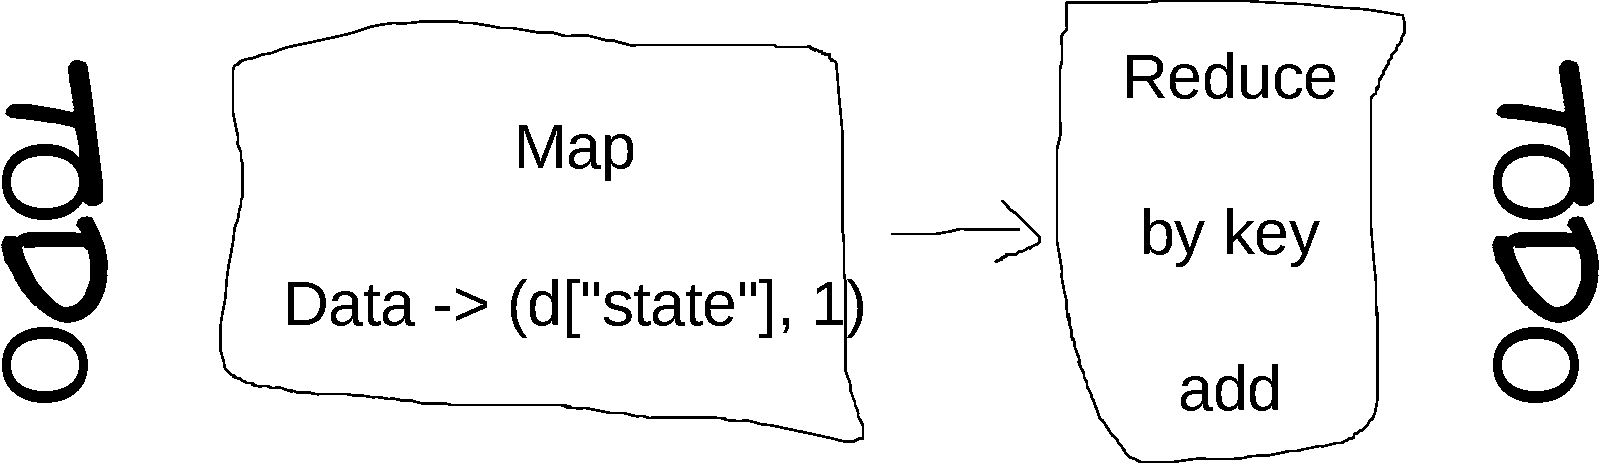
\includegraphics[width=0.8\textwidth]{assets/images/eval-rq1-mapreduce.pdf}
	\caption{MapReduce pipeline to find the failed runs}
	\label{fig:eval-mapreduce-1}
\end{figure}

\begin{figure}[htbp!]
	\centering
	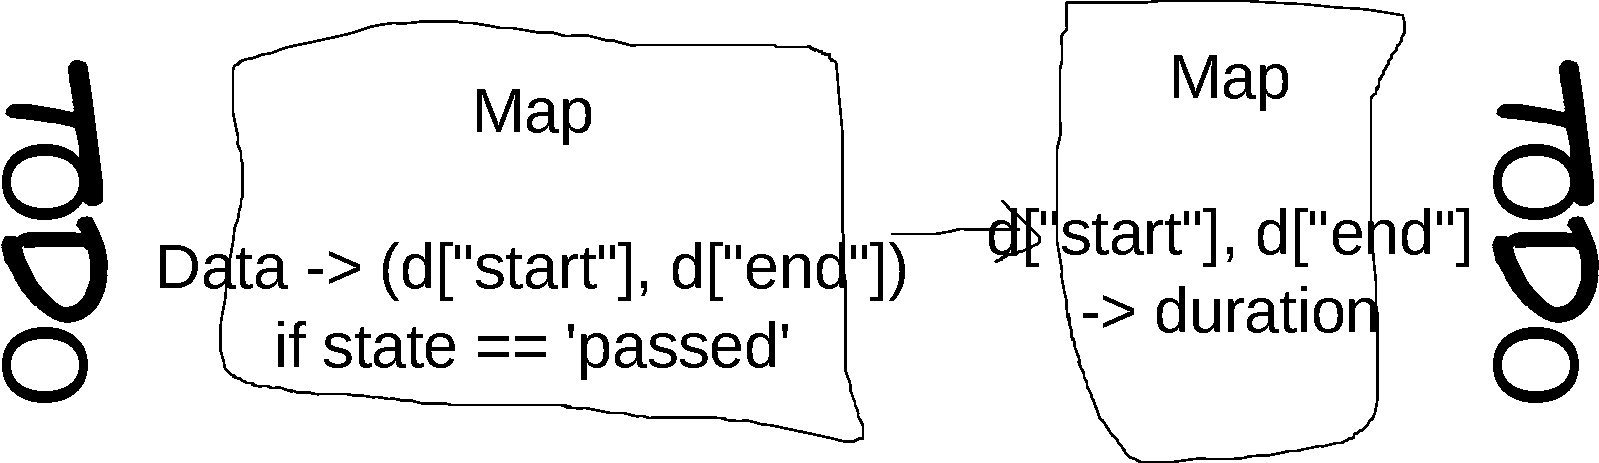
\includegraphics[width=0.8\textwidth]{assets/images/eval-rq3-mapreduce.pdf}
	\caption{MapReduce pipeline to find the average duration of a successful test run}
	\label{fig:eval-mapreduce-3}
\end{figure}

\noindent In addition to the first source, another $\SI{3702595}{}$ jobs have been analysed from the \emph{TravisTorrent} project. This project \cite{msr17challenge} scrapes the API of \travisci{} and combines this with data obtained from the \github{} API to augment the dataset with extra information. One of these additional values is the identifier of the previous executed build of every project. This identifier is required to answer the second research question. Furthermore, the amount of failed test cases in every run is included, which can be used to distinguish whether the test run has actually failed or the project could not be compiled and thus allowing a more fine-grained answer to the first research question as well. After analysis of this dataset, the execution time was not accurate compared to the actual timings on the \travisci{} build page, so this dataset was not used in the third research question. For analysis, the creators of TravisTorrent have provided a Google BigQuery\footnote{\url{https://bigquery.cloud.google.com/}} interface to allow querying the dataset, which is required given its magnitude. The following queries have been executed to obtain the required data:

\lstinputlisting[caption=TravisTorrent query: Find the amount of failed runs, label=lst:travistorrent-sql1, language=sql]{assets/listings/travistorrent-failed-runs.sql}
\lstinputlisting[caption=TravisTorrent query: Find the probability of consecutive failures,label=lst:travistorrent-sql2, language=sql]{assets/listings/travistorrent-consecutive-failures.sql}
